\tikzstyle{selected}=[draw=green,fill=green!30]
\centering
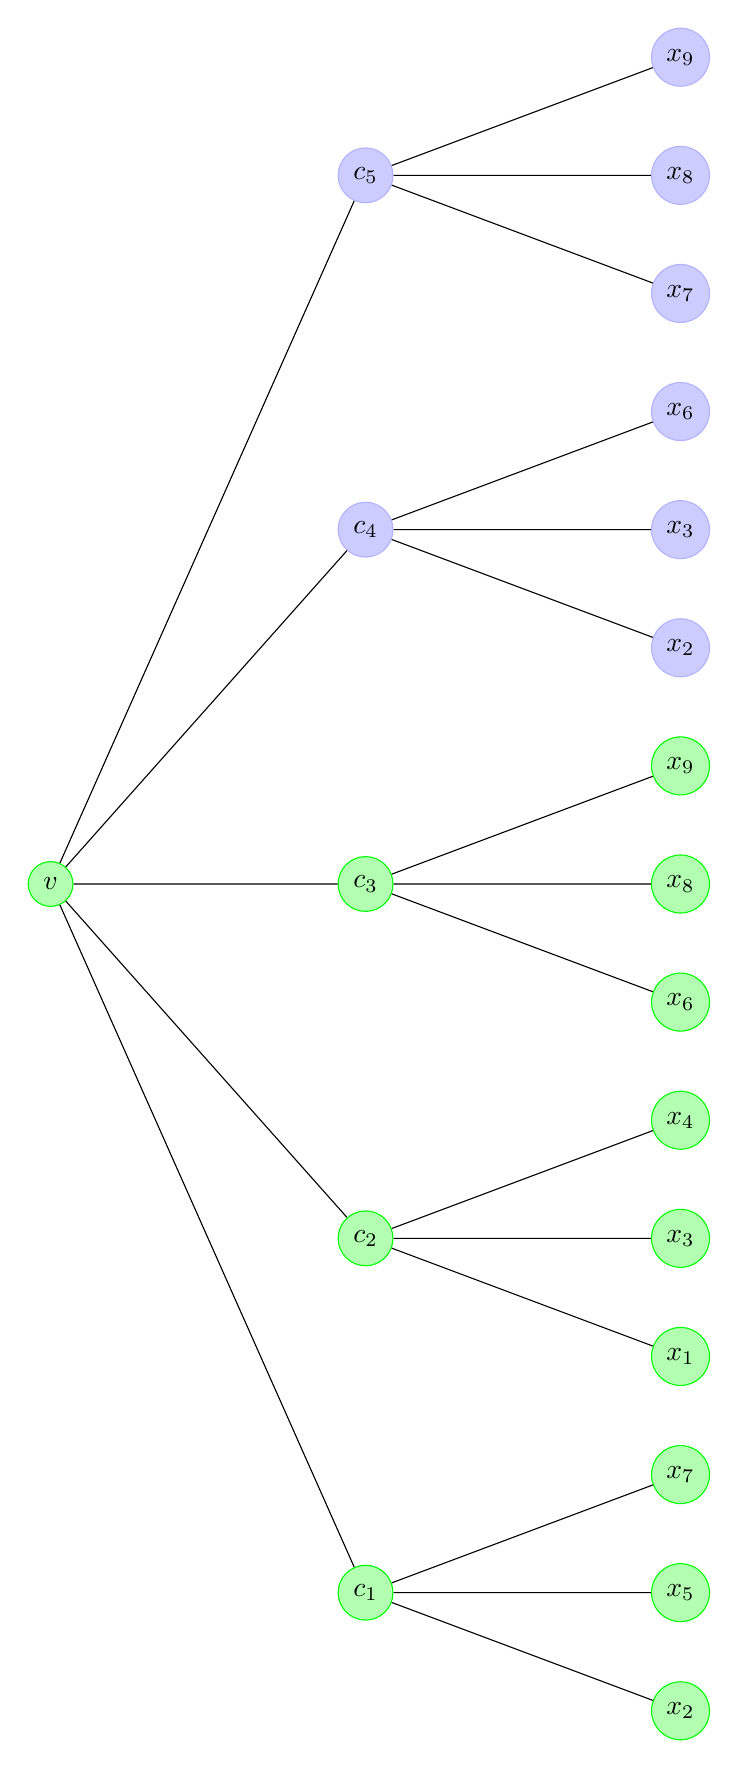
\begin{tikzpicture}[grow = 0, nodes={draw=blue!30, circle, fill=blue!20}, level distance=4cm]
\node [selected] {$v$}
  child {
      node [selected] {$c_1$}
      child {node [selected] {$x_2$}}
      child {node [selected] {$x_5$}}
      child {node [selected] {$x_7$}}
    }
    child [missing]
    child [missing]
    child {
      node [selected] {$c_2$}
      child {node [selected] {$x_1$}}
      child {node [selected] {$x_3$}}
      child {node [selected]  {$x_4$}}
    }
    child [missing]
    child [missing]
    child {
      node [selected] {$c_3$}
      child {node [selected] {$x_6$}}
      child {node [selected] {$x_8$}}
      child {node [selected] {$x_9$}}
    }
    child [missing]
    child [missing]
    child {
      node {$c_4$}
      child {node {$x_2$}}
      child {node {$x_3$}}
      child {node {$x_6$}}
    }
    child [missing]
    child [missing]
    child {
      node {$c_5$}
      child {node {$x_7$}}
      child {node {$x_8$}}
      child {node {$x_9$}}
    };
\end{tikzpicture}
